\chapter{Heat Transport in Stratified Atmospheres at low and high Mach number}
\label{ch:ab17}

\section{Preamble}
The following work is the culmination of my comprehensive exam II research and was published in Physical Review Fluids \citep{anders&brown2017}.
The text in section \ref{sec:ab17_published} is the text of the paper as it was accepted for publication.
Following the published work, in section \ref{sec:ab17_postscript}, I comment on a few lessons that have been learned since we published these results.

This work was motivated in large part by the study of \citet{brandenburg&all2005} and conversations with Axel Brandenburg and Ben Brown.
In Axel's 2005 work, he argues that the superadiabatic excess, $\epsilon$, defined below near Eqn.~\ref{eqn:polytrope}, should be large if one aims to study astrophysical convection.
He finds in his experiments that, as $\epsilon$ grows, the fraction of the system flux carried by the evolved convection approaches unity.
However, we knew that as $\epsilon$ grows, so too does the Mach number of the convection.
We were convinced that low $\epsilon$ polytropes were an ideal experimental setup in which to study low Mach number, stratified convection.
Furthermore, the radiative background flux carried by the background adiabat in polytropes \emph{does not interact with the nonlinear flows}.
It is to first order in hydrostatic and thermal equilibrium, and so it should ``fall out'' of the equations of motion.

Despite our conviction that low $\epsilon$ and high $\epsilon$ convection were both valid convective experiments, we had no way to \emph{prove} that was the case.
In this work, we came to a more full understanding of how to define the Nusselt number in compressible flows, and we found that---indeed---a properly defined measure of the convective flux (Nu) scales similarly at low and high $\epsilon$.
This suggests that, regardless of $\epsilon$, properly measured convection in a polytrope can sample the nature of turbulent convective flows as the convective driving (Rayleigh number) is increased.


\section{Published work}
\label{sec:ab17_published}

\subsection{Introduction}
\label{sec:intro}
Convection transports energy in stellar and planetary atmospheres where flows are compressible and feel the atmospheric stratification.  
This stratification is significant in regions such as the convective envelope of the Sun, which spans 14 density scale heights.
In the bulk of these systems, particularly in the deep interior, flows are at very low Mach number (Ma).  
Unfortunately, numerical constraints have restricted most studies of compressible convection to high Ma.
These prior studies \citep{graham1975, chan&all1982, hurlburt&all1984, cattaneo&all1990, brummell&all1996, brandenburg&all2005} have provided insight into the nature of convection in the low temperature, high Ma region near the Sun's surface. 
Few fundamental properties of low Ma compressible convection, such as the scaling of convective heat transport, are known.

In the widely-studied \RB problem of incompressible Boussinesq convection (RBC), a sufficiently negative temperature gradient causes convective instability.
In the evolved solution, upflows and downflows are symmetrical, the temperature in the interior becomes isothermal, and the conductive flux ($\propto \grad T$) approaches zero there. 
For compressible convection in a stratified atmosphere, a negative entropy gradient causes convective instability.
Early numerical experiments of moderate-to-high Ma compressible convection in two \citep{graham1975, chan&all1982, hurlburt&all1984, cattaneo&all1990} and three \citep{cattaneo&all1991, brandenburg&all2005, brummell&all1996} dimensions revealed a different evolved state from RBC.
Downflow lanes become fast and narrow, and upflow lanes turn into broad, slow upwellings.
Furthermore, the \emph{entropy} gradient is negated by convection in the interior, so a significant temperature gradient and conductive flux can persist despite efficient convection.

In RBC, there exist two primary dynamical control parameters: the Rayleigh number (Ra, the ratio of buoyant driving to diffusive damping) and the Prandtl number (Pr, the ratio of viscous to thermal diffusivity). 
These numbers control two useful measures of turbulence in the evolved solution: the Reynolds number (Re, the strength of advection to viscous diffusion) and the Peclet number (Pe, advection vs. thermal diffusion).  
In stratified atmospheres, the magnitude of the unstable entropy gradient joins Ra and Pr as a third important and independent control parameter.  
This \emph{superadiabatic excess}, $\epsilon$, sets the scale of the atmospheric entropy gradient \citep{graham1975}.
We find here that $\epsilon$ primarily controls the Ma of the evolved solution.

Here we study the behavior of convective heat transport, quantified by the Nusselt number (Nu), in plane-parallel, two- and three-dimensional, polytropically stratified atmospheres.  
We vary $\epsilon$ and Ra while holding Pr, aspect ratio, boundary conditions, and initial atmospheric stratification constant.  
We also examine the behavior of flow properties, as quantified by Ma and Re.
We find here that the scaling of Nu in stratified, compressible convection is similar to that in \RB convection, and that this scaling is not appreciably changed by the magnitude of the superadiabaticity.

\subsection{Experiment} 
\label{sec:experiment}
We examine a monatomic ideal gas with an adiabatic index of $\gamma = 5/3$ whose equation of state is $P = R\rho T$. 
This is consistent with the approach used in earlier work \citep{graham1975, chan&all1982, brandenburg&all2005, hurlburt&all1984, cattaneo&all1990, cattaneo&all1991, brummell&all1996}  and is the simplest stratified extension of RBC.
The atmospheres studied here are initially polytropically stratified,
\begin{equation}
\begin{split}
\rho_0(z) &= \rho_{t}(1 + L_z - z)^m, \\
T_0(z)    &= T_{t}(1 + L_z - z),
\label{eqn:polytrope}
\end{split}
\end{equation}
where $m$ is the polytropic index and $L_z$ is the depth of the atmosphere.
The polytropic index is set by the superadiabatic excess, $\epsilon = m_{ad} - m$, where $m_{ad} = (\gamma - 1)^{-1}$ is the adiabatic value of $m$.
The height coordinate, $z$, increases upwards in the range $[0, L_z]$.
Subscript 0 indicates initial conditions and subscript $t$ indicates values at $z = L_z$.   
Stratified atmospheres have a fourth non-dimensional parameter, the number of density scale heights, $n_{\rho} = \ln\left[\rho_0(z=0)/\rho_t\right]$.  
We specify the depth of the atmosphere, $L_z = e^{n_{\rho}/m} - 1$, by choosing the initial value of $n_{\rho}$.
Throughout this work we set $n_{\rho} = 3$.    Satisfying hydrostatic equilibrium sets the value of gravity, $g = RT_t (m + 1)$, which is constant with depth.  
We study atmospheres with aspect ratios of 4 where both the $x$ and $y$ coordinates have the range $[0, 4L_z]$.
In our 2D cases, we only consider $x$ and $z$.

These domains are nondimensionalized by setting $R = T_t = \rho_t = 1$ at $z = L_z$.
By this choice, the non-dimensional length scale is the inverse temperature gradient scale and the timescale is the isothermal sound crossing time, $\tau_I$, of this unit length.
Meaningful convective dynamics occur on timescales of the atmospheric buoyancy time, $t_b = \tau_I \sqrt{L_z\,m\,c_P/g\,\epsilon\,n_\rho}$, where $c_P = R \gamma/(\gamma-1) = 2.5$ is the specific heat at constant pressure.

At fixed $n_\rho$, convective dynamics are controlled by $\epsilon$ as well as the atmospheric diffusivities.
At a fixed value of $\epsilon$, the diffusivities are set by the Rayleigh number (Ra) and the Prandtl number (Pr),
\begin{equation}
\text{Ra}_{t} = \frac{g L_z^3 (\Delta S_0 / c_P)}{\nu_t\chi_t},
\qquad
\text{Pr} = \frac{\nu}{\chi},
\end{equation}
where $\Delta S_0 = \epsilon\ln (1 + L_z) = \epsilon n_\rho / m$ is the initial specific entropy difference across the domain, $\chi$ is the thermal diffusivity, and $\nu$ is the kinematic viscosity.
Throughout this work we specify that Pr $= 1$ and is depth invariant.
The initial thermal conductivity, $\kappa_0 = \chi \rho_0$, is constant with depth, such that (\ref{eqn:polytrope}) is in thermal equilibrium ($\grad\cdot[\kappa_0\grad T_0] = 0$).
By these choices, $\nu(z) \equiv \chi(z) \equiv \chi_t / \rho_0$.
This formulation sets Ra at the bottom of the domain greater than Ra$_t$ by a factor of $e^{2n_\rho}$. 
Henceforth when we specify Ra we are referring to Ra$_t$.  
The full values of $\kappa = \rho\chi$ and $\mu = \rho\nu$ (the dynamic viscosity) change as the density profile evolves.  
The diffusivities scale as $\chi_t, \nu_t \propto \sqrt{g L_z^3 (\Delta S_0 / c_P) / \text{Ra}_t}$.
Defining the thermal diffusion timescale as $t_\chi \equiv \tau_IL_z^2 / \chi$, the ratio of $t_\chi$ to the buoyancy time is
\begin{equation}
\frac{t_\chi}{t_b} =\text{Ra}_t^{1/2}.
\label{eqn:timescales}
\end{equation}
We carry out two experiments in this study. 
In the first, we fix $\epsilon$ and increase Ra, thus increasing the ratio in (\ref{eqn:timescales}). 
In the second, we fix Ra and vary $\epsilon$, scaling the dynamical timescales $(t_b, t_\chi)$ as $\epsilon^{-1/2}$ relative to the speed of sound; we see this reflected in the evolved Mach number scaling (Fig. \ref{fig:ma_v_eps}).

We use $\ln \rho$ and $T$ as our thermodynamic variables and solve the Fully Compressible Navier-Stokes equations,
\begin{align}
&\begin{aligned}
&\frac{\partial \ln\rho}{\partial t} + \grad\cdot\bm{u} 
    = -\bm{u}\cdot\grad\ln\rho,
	\label{eqn:continuity_eqn}
\end{aligned}\\
&\begin{aligned}
\frac{\partial\bm{u}}{\partial t} + \grad T - 
&\nu\grad\cdot\lilstressT - \lilstressT\cdot\grad\nu =
-\bm{u}\cdot\grad\bm{u} - T\grad\ln\rho + \bm{g} + 
\nu\lilstressT\cdot\grad\ln\rho,
\label{eqn:momentum_eqn}
\end{aligned}\\
&\begin{aligned}
\frac{\partial T}{\partial t} -\frac{1}{c_V}\left(\right.\chi&\left.
    \grad^2 T + \grad T\cdot\grad\chi\right) =
	-\bm{u}\cdot\grad T - (\gamma-1)T\grad\cdot{\bm{u}}
	+ \frac{1}{c_V}\left(\chi\grad T \cdot\grad\ln\rho +
	\nu\left[\lilstressT\cdot\nabla\right]\cdot\bm{u}\right), 
	\label{eqn:energy_eqn}
\end{aligned}
\end{align}
with the viscous stress tensor given by
\begin{equation}
\sigma_{ij} \equiv \left(\frac{\partial u_i}{\partial x_j} + 
\frac{\partial u_j}{\partial x_i} - \frac{2}{3}\delta_{ij}\grad\cdot\bm{u}\right),
	\label{eqn:stress_tensor}
\end{equation}
where $\delta_{ij}$ is the Kronecker delta. 
Taking an inner product of (\ref{eqn:momentum_eqn}) with $\rho\bm{u}$ and adding it to $\rho c_V\times$(\ref{eqn:energy_eqn}) reveals the full energy equation,
\begin{equation}
\frac{\partial}{\partial t}\left(\rho\left[\frac{|\bm{u}|^2}{2} + c_V T + \phi\right]\right) +
\Div{\bm{F}_{\text{conv}} + \bm{F}_{\text{cond}}} = 0,
	\label{eqn:energy_eqn_full}
\end{equation}
where
$
\bm{F}_{\text{conv}} \equiv \bm{F}_{\text{enth}} + \bm{F}_{\text{KE}} + \bm{F}_{\text{PE}} + \bm{F}_{\text{visc}}
$
is the convective flux and $\bm{F}_{\text{cond}} = -\kappa \grad T$ is the conductive flux.
The individual contributions to $\bm{F}_{\text{conv}}$ are the enthalpy flux, $\bm{F}_{\text{enth}} \equiv \rho\bm{u}(c_V T + P/\rho)$; the kinetic energy flux, $\bm{F}_{\text{KE}} \equiv \rho|\bm{u}|^2\bm{u}/2$; the potential energy flux, $\bm{F}_{\text{PE}} \equiv \rho\bm{u}\phi$ (with $\phi \equiv -gz$); and the viscous flux, $\bm{F}_{\text{visc}} \equiv -\rho\nu\bm{u}\cdot\lilstressT$.
Understanding how each of these fluxes interact is crucial in characterizing convective heat transport.

We utilize the Dedalus\footnote{\url{http://dedalus-project.org/}} pseudospectral framework \citep{burns&all2016} to time-evolve (\ref{eqn:continuity_eqn})-(\ref{eqn:energy_eqn}) using an implicit-explicit (IMEX), third-order, four-step Runge-Kutta timestepping scheme RK443 \citep{ascher&all1997}.  
Thermodynamic variables are decomposed such that $T = T_0 + T_1$ and $\ln\rho = (\ln\rho)_0 + (\ln\rho)_1$, and the velocity is $\bm{u} = w\bm{\hat{z}} + u\bm{\hat{x}} + v\bm{\hat{y}}$.
In our 2D runs, $v = 0$.
Subscript 0 variables, set by (\ref{eqn:polytrope}), have no time derivative and vary only in $z$.
Variables are time-evolved on a dealiased Chebyshev (vertical) and Fourier (horizontal, periodic) domain in which the physical grid dimensions are 3/2 the size of the coefficient grid.  
Domain sizes range from 64x256 coefficients at the lowest values of Ra to 1024x4096 coefficients at Ra $> 10^{7}$ in 2D, and from 64x128$^2$ to 256x512$^2$ in 3D. 
By using IMEX timestepping, we implicitly step the stiff linear acoustic wave contribution and are able to efficiently study flows at high ($\sim 1$) and low ($\sim 10^{-4}$) Ma.  
Our equations take the form of the FC equations in \cite{lecoanet&all2014}, extended to include $\nu$ and $\chi$ which vary with depth, and we follow the approach there.
This IMEX approach has been successfully tested against a nonlinear benchmark  of the compressible Kelvin-Helmholtz instability \citep{Lecoanet_et_al_2016_KH}.

We impose impenetrable, stress free, fixed temperature boundary conditions at the top and bottom of the domain, with $w = \partial_z u = T_1 = 0$ at $z = \{0, L_z\}$. 
$T_1$ is initially filled with random white noise whose magnitude is infinitesimal compared to $\epsilon T_0$.
We filter this noise spectrum in coefficient space, such that only the lower 25\% of the coefficients have power. 
All reported results are taken from time averages over many $t_b$ beginning \{100, 40\}$t_b$ after the start of our \{2D, 3D\} simulations to ensure our results are not biased by the convective transient.

\subsection{Results \& Discussion}
\label{sec:results}


\begin{figure}[t]
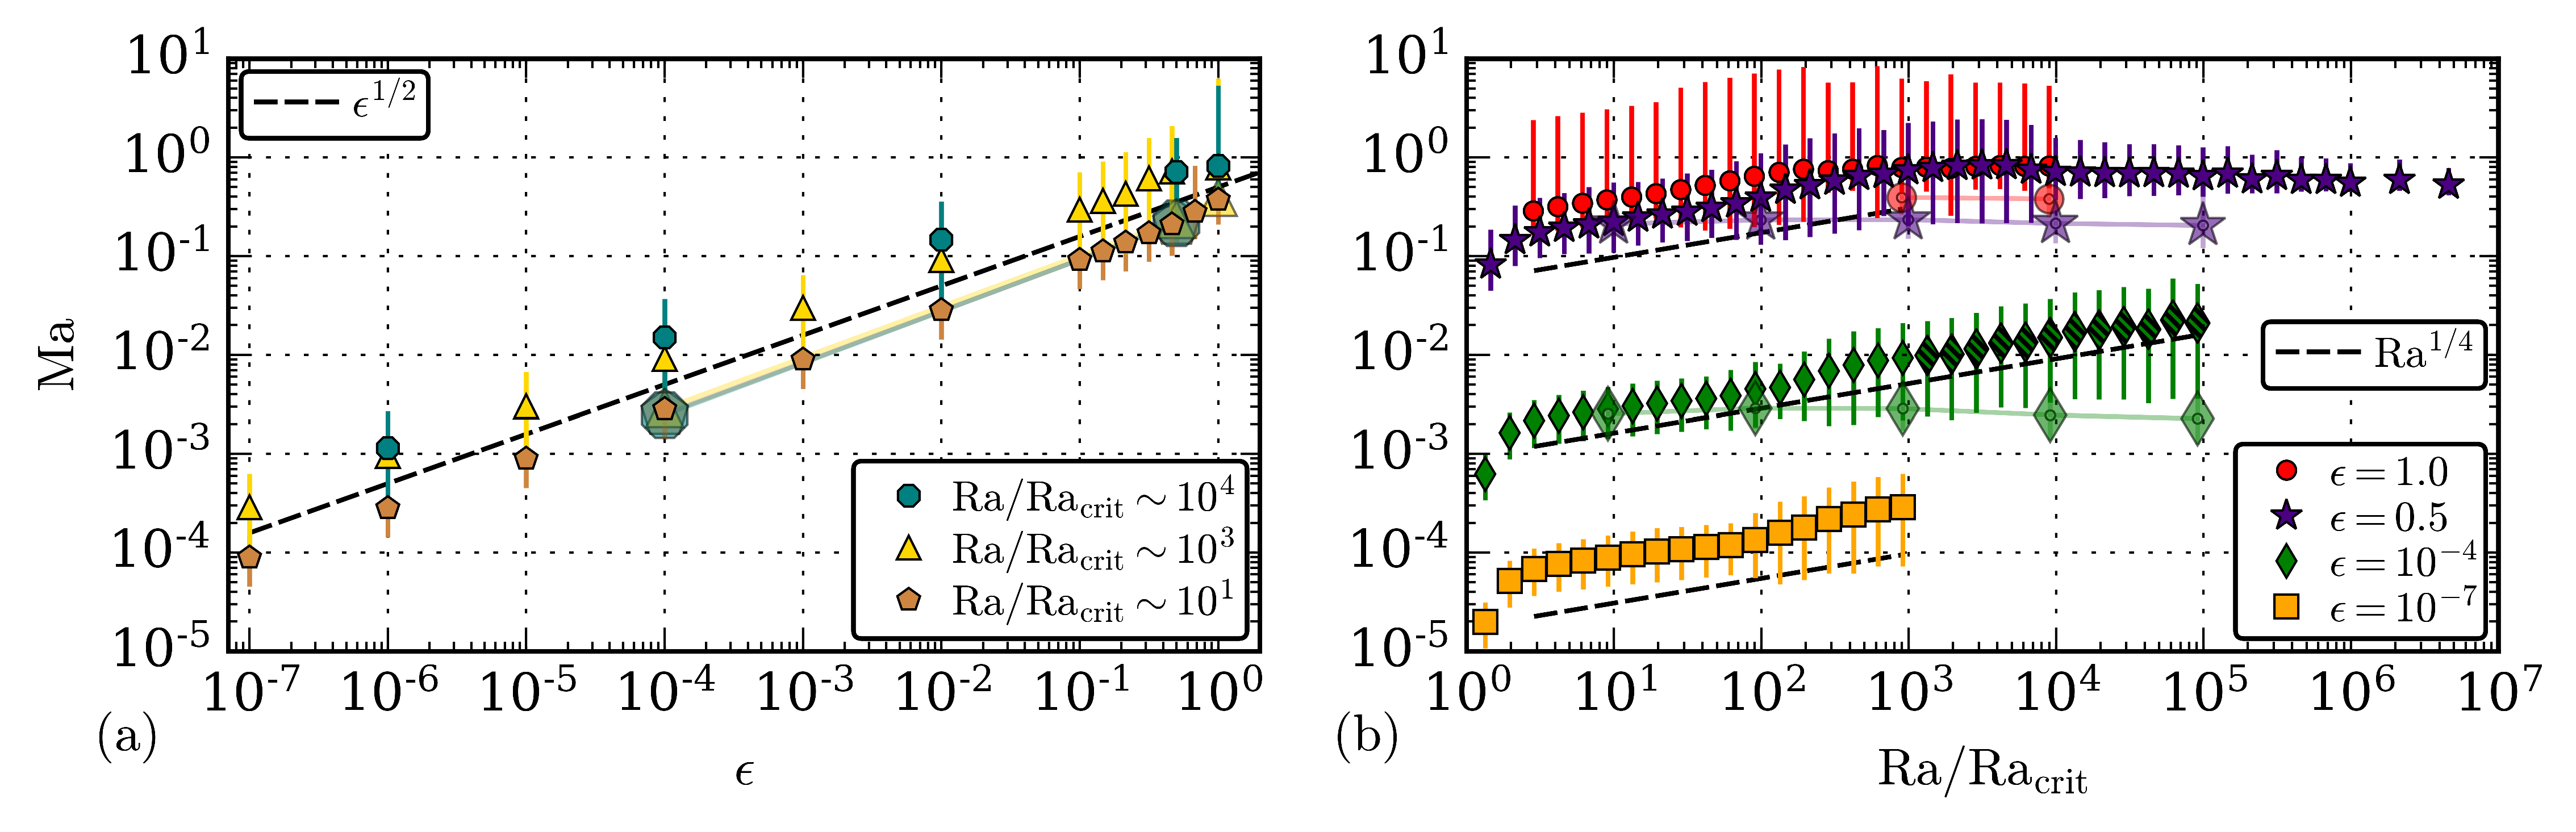
\includegraphics[width=\textwidth]{./figs/ma_v_Ra.pdf}
\caption[Mach number scaling in polytropic solutions.]
{
	The mean adiabatic Mach number of long-time-averaged profiles is shown.  
	Error bars show the full range of Ma over the depth of the atmosphere.
	(a) Ma, at various values of Ra, is plotted as a function of $\epsilon$.
	(b) Ma, at various values of $\epsilon$, is plotted as a function of Ra/Ra$_{\text{crit}}$.
	Larger symbols with inlaid circles designate 3D runs.
	\label{fig:ma_v_eps} 
}
\end{figure}


Solutions were time-evolved until a long time average of the fluxes showed little variance with depth.
A linear stability analysis determined that convective onset occurs at $\text{Ra}_{\text{crit}} = \{11.15, 10.06, 10.97, 10.97\}$ for $\epsilon = \{1.0, 0.5, 10^{-4}, 10^{-7}\}$, respectively.  

\subsubsection{Evolved fluid numbers \& flow morphology}

We measure the adiabatic Mach number (Ma = $|\bm{u}|/\sqrt{\gamma T}$), and find that it is a strong function of $\epsilon$ and a weak function of Ra.  
In our 2D runs, when Ma $< 1$, we observe a scaling law of Ma(Ra$, \epsilon) \appropto \epsilon^{1/2}$Ra$^{1/4}$.
This relation breaks down as the mean Ma approaches 1 (Fig. \ref{fig:ma_v_eps}).  
This transition occurs near Ra/Ra$_\text{crit} \approx \{10^{2}, 10^{3}\}$ for $\epsilon = \{1, 0.5\}$.
In our limited 3D runs, Ma appears to be a function of $\epsilon$ alone, with Ma $\appropto \epsilon^{1/2}$, so at high Ra, Ma$_{\text{3D}} < \text{Ma}_{\text{2D}}$.
We conjecture that the scaling of Ma with Ra in the 2D runs is due to the formation of coherent high-velocity ``spinners,'' which form between upflow and downflow lanes.  
These structures, which are reminiscent of flywheel modes in RBC, do not appear in our 3D runs at these parameters \citep{jones&all1976, brummell&all2002}.
Simulations in the range of Ra/Ra$_{\text{crit}} > 10^3$ at $\epsilon = 10^{-4}$ exhibited ``windy'' states of convection, in which a large-scale horizontal shearing flow replaced the more standard upflow/downflow morphology of convection.  
Similar states have been studied in RBC \citep{goluskin&all2014}.  
These runs are represented in Figs.~\ref{fig:ma_v_eps}, \ref{fig:re_and_nu_v_ra}, \& \ref{fig:nrho_v_ra} as hatched points, and while this phenomenon does not appear to greatly modify the scaling of fluid properties measured in this work, these states warrant further investigation.

In 2D, low Ma flows (e.g., $\epsilon = 10^{-4}$) display the classic narrow downflow and broad upflow lanes of stratified convection (Fig. \ref{fig:entropy_snapshots}a).
At high Ma (e.g., $\epsilon = 0.5$, Ra/Ra$_{\text{crit}} \gtrsim 10^3$), bulk thermodynamic structures are similar but shock systems form in the upper atmosphere near downflow lanes (Fig. \ref{fig:entropy_snapshots}b\&c), as reported previously \citep{cattaneo&all1990, malagoli&all1990}.
At large Ra, the diffusion timescale becomes long (\ref{eqn:timescales}), and thermodynamic structures form small eddies which traverse the domain repeatedly before diffusing (Fig. \ref{fig:entropy_snapshots}c).
As evidenced by the colorbar scalings, the amplitudes of thermodynamic fluctuations scale with $\epsilon$.

In 3D, the same upflow/downflow asymmetry is seen, but other aspects of the flow are distinctly different.  
Fig. \ref{fig:entropy_snapshots}d-f show select snapshots of a 3D simulation with the same input parameters as the 2D case in Fig. \ref{fig:entropy_snapshots}a.
In 2D, large-scale, coherent spinners dominate the  flow, leading to a single upflow and downflow.  
New downflowing plumes at the upper boundary are efficiently swept into the large coherent structure (near $x \sim 1$ and spanning the vertical domain).  
The behavior of downflows in 3D is strikingly different (Fig. \ref{fig:entropy_snapshots}d).
In 3D, many individual plumes detach from the upper boundary, but do not organize into a single dominant downflow in the same fashion.  
Horizontal cuts near the top of the domain (Fig. \ref{fig:entropy_snapshots}e) reveal a network of narrow downflow lanes surrounding broad upflows. 
Stronger clusters of downflows near the surface are linked to sheets of low entropy at the midplane of the domain (Fig. \ref{fig:entropy_snapshots}f).
As the flows evolve in time, new downflows appear at the top of the domain in the middle of upflows and join the surrounding downflow network, causing the convective structures to fragment.  
There is no preferred orientation in the newly forming downflows, and the convective flow field constantly evolves, which appears to prevent the occurrence of either spinners or windy states.

\begin{figure}[t!]
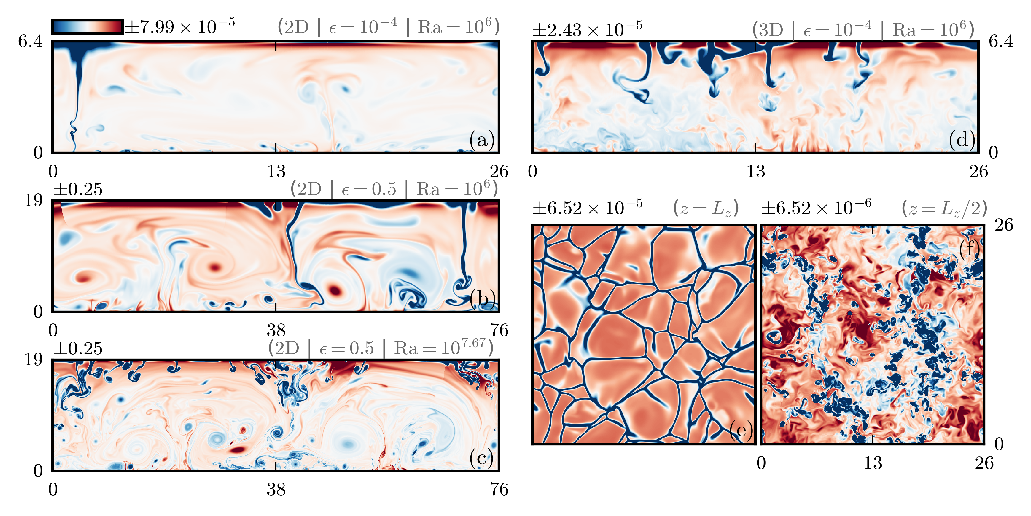
\includegraphics[width=\textwidth]{./figs/snapshots_fig_raster.pdf}
\caption[Flow morphology of 2D, 3D, and low and high Mach number flows.]
{
	Characteristic entropy fluctuations in evolved flows roughly $\{$140, 60$\}$ $t_b$ after the start of simulations for $\{$2D, 3D$\}$ runs. 
	The time- and horizontally-averaged profile is removed in vertical slices (a)-(d). 
	The time- averaged mean value is removed in horizontal slices (e) and (f).
	(a) A low Ma flow at moderate Ra. 
	(b) A high Ma flow at the same Ra as in (a).
	(c) A high Ma flow at high Ra. 
	Shock systems can be seen in the upper atmosphere of the high Ma flows, for example at $(x, z) \sim (5, 15-19)$ in (b) and $(x, z) \sim (50, 15-19)$ in (c).
	(d)-(f) A low Ma 3D run at the same parameters as in (a), where (d) is a vertical ($x$, $z$) slice at $y = L_y/2$, (e) is a horizontal slice at $z = L_z$, and (f) is a horizontal slice at $z = L_z/2$.
	\label{fig:entropy_snapshots} 
}
\end{figure}



The efficiency of convection is quantified by the Nusselt number (Nu).  
Nu is well-defined in RBC as the total flux normalized by the steady-state conductive flux \citep{johnston&doering2009, otero&all2002}.
In stratified convection Nu is more difficult to define, and we use a modified version of a traditional stratified Nusselt number \citep{graham1975,hurlburt&all1984},
\begin{equation}
\text{Nu} \equiv \frac{\langle F_{\text{conv,z}} + F_{\text{cond,z}} - F_{\text{A}}\rangle}
{\langle F_{\text{cond,z}} - F_{\text{A}}\rangle} 
= 1 + \frac{\langle F_{\text{conv,z}}\rangle}{\langle F_{\text{cond,z}} - F_{\text{A}} \rangle}
\label{eqn:nusselt}
\end{equation}
where $F_{\text{conv,z}}$ and $F_{\text{cond,z}}$ are the z-components of $\bm{F}_{\text{conv}}$ and $\bm{F}_{\text{cond}}$, and $\langle \rangle$ are volume averages.  
$F_{\text{A}} \equiv -\langle\kappa\rangle \partial_z T_{\text{ad}}$ is the conductive flux of the proper corresponding adiabatic atmosphere.
For a compressible, ideal gas in hydrostatic equilibrium, $\partial_z T_{\text{ad}} \equiv - g / c_{P}$ \citep{spiegel&veronis1960}.  
It is important to measure the evolved value of $\langle \kappa \rangle = \langle \rho\chi \rangle$, which is nearly $\kappa_0$ for small $\epsilon$ but changes appreciably for large values of $\epsilon$.
In incompressible Boussinesq convection, where $\grad S = 0$ only when $\grad T = 0$, and where $\kappa$ is constant with depth and time, this definition reduces to the traditionally defined Nusselt number \citep{otero&all2002, johnston&doering2009}.
\begin{figure}[t!]
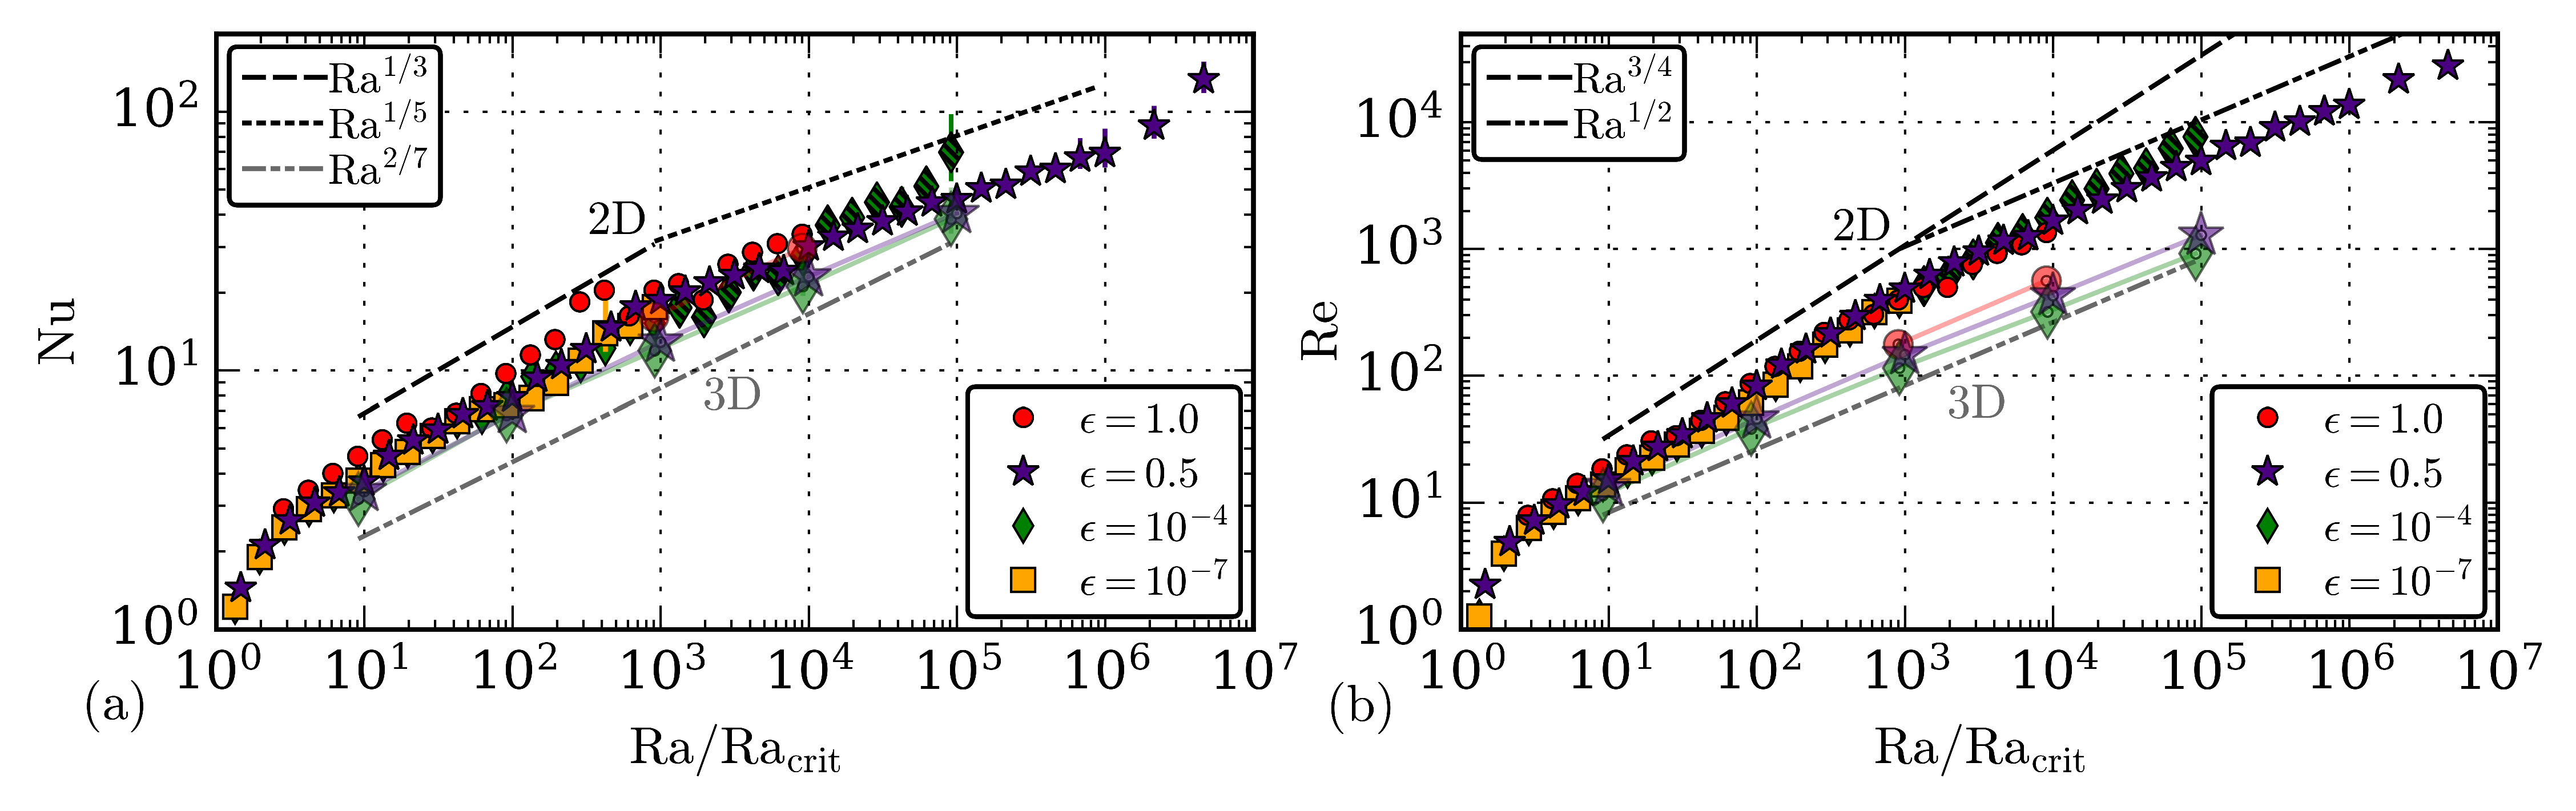
\includegraphics[width=\textwidth]{./figs/re_and_nu_v_Ra.pdf}
\caption[Scaling of Nusselt and Reynolds number at low and high Mach number.]
{
	Flow properties at high and low $\epsilon$. 
	(a) Nu vs. Ra/Ra$_{\text{crit}}$.
	Errors bars indicate the variance of Nu with depth; large error bars indicate a poorly converged solution.
	(b) Re vs. Ra/Ra$_{\text{crit}}$.
	Re is measured at the midplane of the atmosphere.
	Larger symbols with inlaid circles designate 3D runs.
	\label{fig:re_and_nu_v_ra}
}
\end{figure}


The variation of Nu with Ra is shown in Fig. \ref{fig:re_and_nu_v_ra}a.  
We find that the Nu depends primarily on Ra, not on $\epsilon$, except where dynamical regimes change.
In 2D and at low to moderate Ra, Nu $\appropto$ Ra$^{1/3}$ regardless of $\epsilon$, reminiscent of scaling laws in \RB boundary layer theory \citep{grossman&lohse2000, ahlers&all2009, king&all2012}.
As the flow becomes supersonic,  Nu $\appropto$ Ra$^{1/5}$.
It is also important to note that, in 2D, the value of Nu is heavily dependent upon the specific thermodynamic structures of the solution, and slight changes in Ra can result in a simulation converging to one solution or another. 
Select simulations were run at higher aspect ratios (8 and 16), and similar flow morphologies were obtained, suggesting that these states are not highly sensitive to aspect ratio.
In our limited 3D runs, it appears that Nu $\appropto$ Ra$^{2/7}$, a classic scaling law seen in RBC \citep{johnston&doering2009}.

The rms Reynolds number (Re = $|\bm{u}|L_z/\nu$) and Peclet number (Pe = Pr Re) compare the importance of advection to diffusion in the evolved convective state.  
For Pr = 1, Pe = Re.  
Our choice of $\{\nu,\chi\}\propto \rho_0^{-1}$ drastically changes the value of Re between the top and bottom of the atmosphere.  
We report values of Re at the midplane ($z=L_z/2$) of the atmosphere in Fig. \ref{fig:re_and_nu_v_ra}b.  
We find that Re depends largely on Ra, but not $\epsilon$, except when the flow regime changes.
In 2D Re $\appropto$ Ra$^{3/4}$ at low Ra.    
When the 2D flows become supersonic,  Re $\appropto$ Ra$^{1/2}$, as expected from (\ref{eqn:timescales}).
In our limited 3D runs, Re $\appropto$ Ra$^{1/2}$, consistent with the supersonic results.
The heightened scaling of Re in 2D follows the scaling of velocity (Ma) with Ra, as seen in Fig. \ref{fig:ma_v_eps}, and reflects the presence of coherent spinners, which do not exist in 3D.

\subsubsection{Evolved stratification}

In the evolved state, the flows can change the density stratification.
In Fig. \ref{fig:nrho_v_ra}a, we measure the time- and horizontally-averaged density profile in two ways. 
Empty symbols show the number of density scale heights between the maximum and minimum of the atmospheric density profile.  
Solid symbols show the number of density scale heights between the top and bottom of the atmosphere. 
We find that near-sonic and supersonic flows support significant, persistent density inversions in the boundary layers, as was reported previously \cite{brandenburg&all2005}.  
This is visible when solid symbols lie below empty symbols.  
We find this in 2D and 3D, even at very large $\epsilon$.  

Sample evolved density profiles are displayed in Fig. \ref{fig:nrho_v_ra}b.
The natural log of the temporally and horizontally averaged density profile, $\ln \rho = \ln \rho_0 + \ln\rho_1$, is displayed for four cases.  
At low $\epsilon$ (dotted green line), the density stratification is, to first order, unchanged from the initial density stratification.  
At high $\epsilon$, in both 2D (solid purple line) and 3D (dashed purple line and dash-dot-dot red line), the evolved stratification differs significantly from the initial state and does not increase monotonically with depth.
To measure the number of density scale heights between two points in the atmosphere, $z_1$ \& $z_2$, we calculate $n_\rho(z_1, z_2) = \ln\rho(z_2) - \ln\rho(z_1)$.  
Thus, the values plotted in Fig. \ref{fig:nrho_v_ra}a for the cases in Fig. \ref{fig:nrho_v_ra}b can be directly read off.  
For example, at $\epsilon = 1$ and Ra/Ra$_{\text{crit}} \sim 10^4$ (dash-dot-dot red line), measuring the stratification between the boundaries retrieves $n_\rho(L_z, 0) \approx -0.3$, but measuring between the maximum and minimum value of the profile retrieves $n_\rho(\text{min, max}) \approx 1.6$.

Surprisingly, the evolved $n_\rho$ is always less than the initial $n_\rho = 3$, and turbulent pressure support plays a larger role than atmospheric slumping.
This appears to arise as a result of convection making the interior isentropic in the presence of fixed-temperature boundary conditions; we expect the behavior of the stratification to be dependent on the choice of thermal boundary conditions.
The agreement of Nu \& Re across $\epsilon$ (Fig. \ref{fig:re_and_nu_v_ra}), particularly at low Ra in which all four of our cases collapse onto a single power law, is striking in light of the vastly different evolved stratifications felt by the flows. 


\begin{figure}[t!]
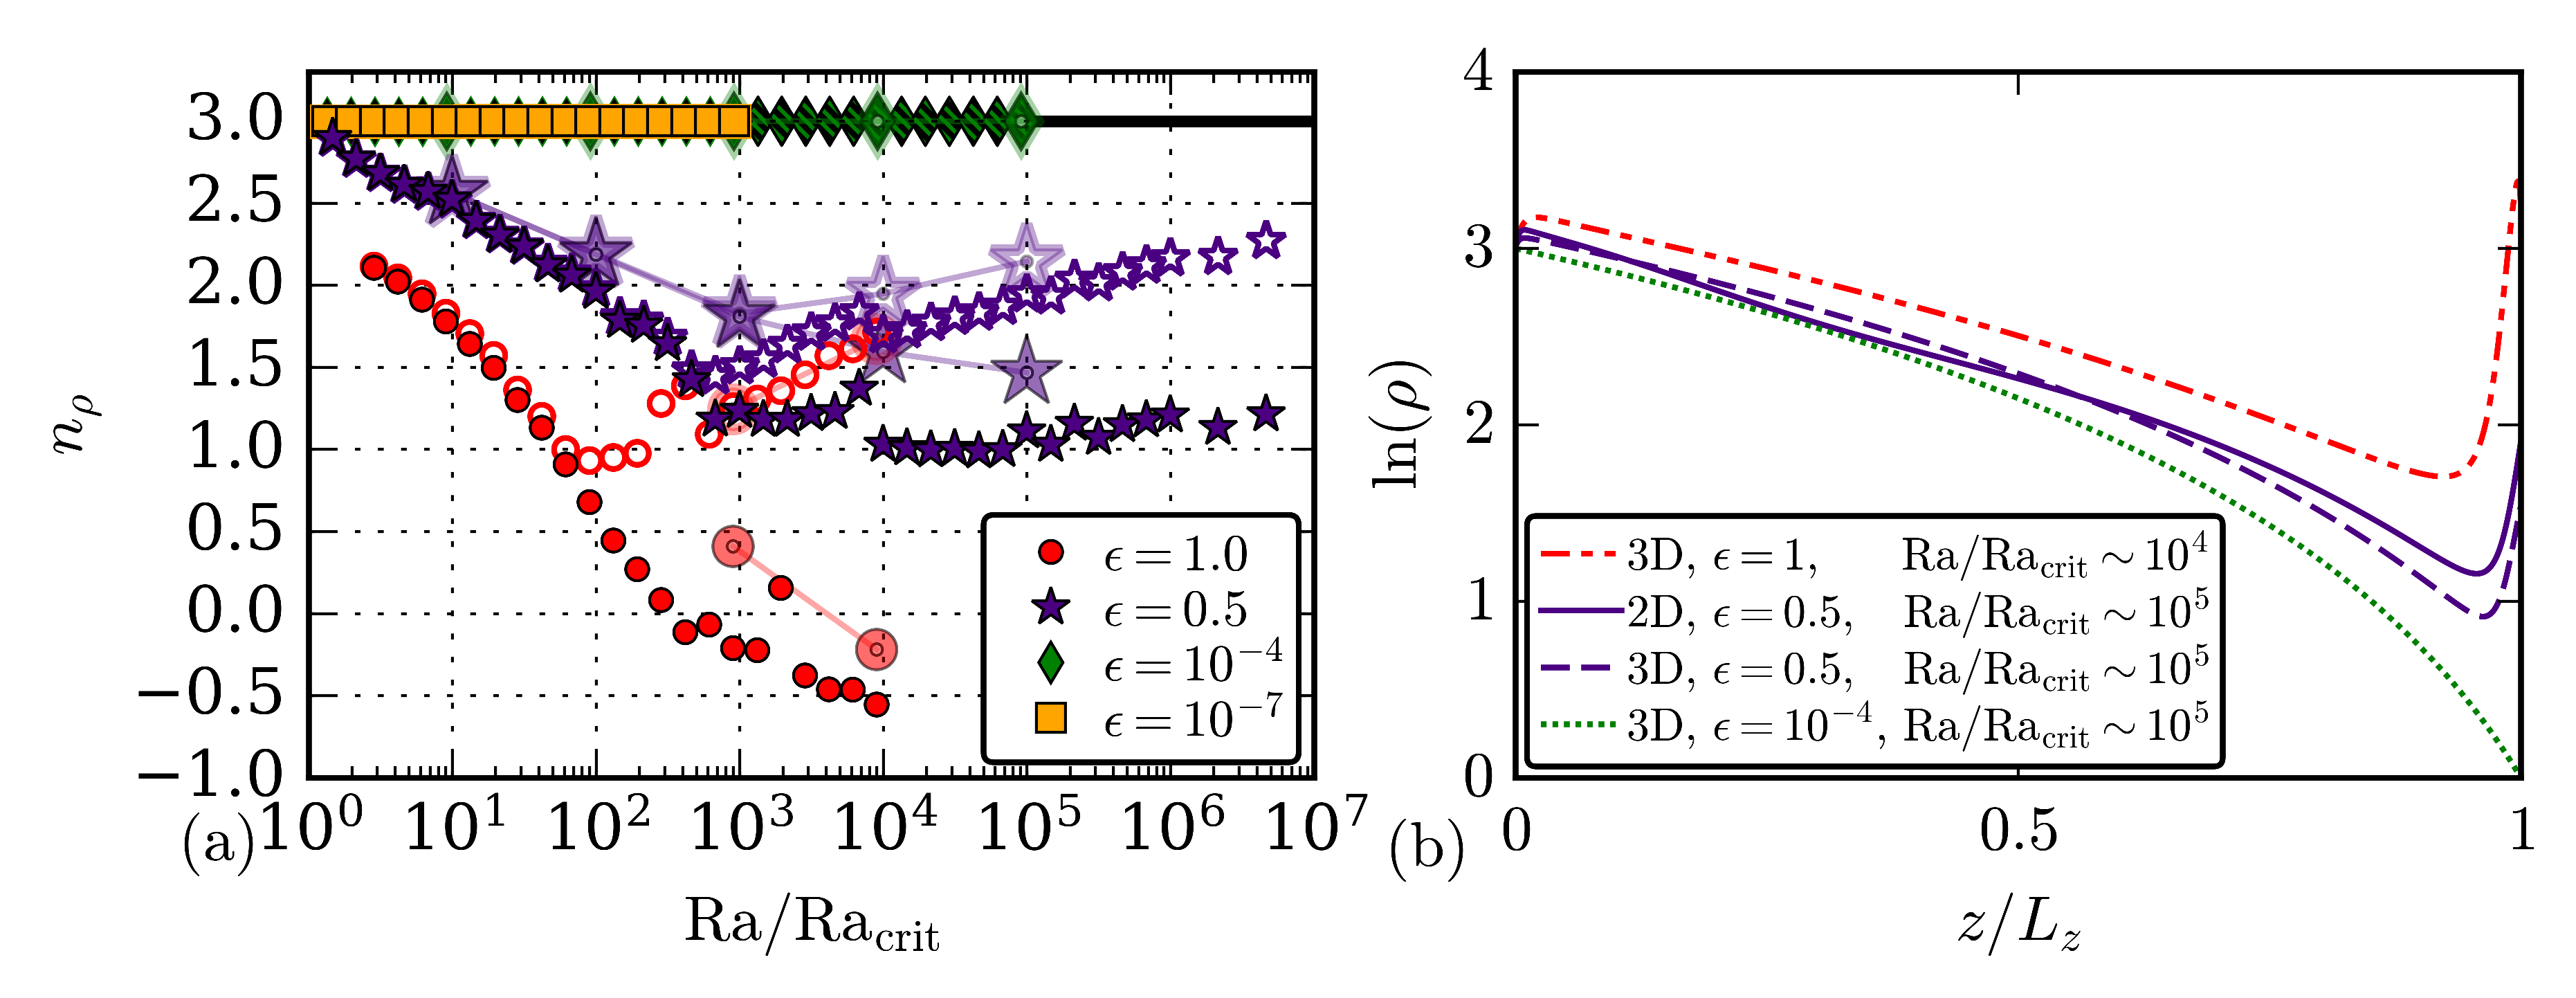
\includegraphics[width=\textwidth]{./figs/density_v_ra.pdf}
\caption[Stratification: density vs.~height at different Mach numbers]
{
	\label{fig:nrho_v_ra} 
	(a) Solid symbols show the density contrast measured in density scale heights between the upper and lower boundary, $n_\rho = \ln[\rho(z=0)/\rho(z=L_z)]$.
	Empty symbols show $n_\rho = \ln[\text{max}(\rho)/\text{min}(\rho)]$. 
	At low $\epsilon$ the evolved $n_{\rho}$ is close to the initial conditions of $n_\rho = 3$.  
	At high $\epsilon$, the density stratification decreases.  
	Once the mean Ma approaches 1 (at Ra/Ra$_{\text{crit}} \approx \{10^2, 10^3\}$ for $\epsilon = \{1, 0.5\}$ as in Fig. \ref{fig:ma_v_eps}b), density inversions form within the thermal boundary layers. 
	Larger symbols represent 3D runs. 
	(b) The natural log of time- and horizontally-averaged density profiles are shown for select simulations, to illustrate the inversions which appear in the boundary layers.
}
\end{figure}

\subsection{Discussion \& Future Work}
We have found that the evolved flow properties of stratified, compressible convection scale in a manner reminiscent of incompressible, Boussinesq \RB convection.
We argue that polytropically stratified atmospheres are the natural extension of the RBC problem with an additional control parameter, $\epsilon$, whose primary role is to set the Ma of the flows.  
We show that other properties of the evolved solutions (Nu, Re) are nearly identical at vastly different values of $\epsilon$, except for where there is a transition between the subsonic and supersonic regimes.  
We also see that Nu scales similarly in 2D and 3D, and that Ma in 3D solutions appears to be a function of $\epsilon$ alone, allowing for simple specification of the evolved Ma using input parameters.
The stratification of these polytropic atmospheres evolves in a complex manner, and future work should aim to understand the importance of stratification on convective heat transport and other flow properties.

Our studies here will serve as a foundation for comparing heat transport in stratified convection to that in RBC \citep{johnston&doering2009} and for better quantifying transport in stratified convection.  
These results can be used to determine if fluid properties scale appropriately in simplified equation sets, such as the anelastic equations.
This work will also be useful in coming to understand more realistic systems, such as rapidly rotating atmospheres \citep{julien&all2012}, atmospheres bounded by stable regions \citep{hurlburt&all1986}, and regions with realistic profiles of $\kappa$.




\subsection{Appendix A: Table of simulation parameters}
In table \ref{table:run_info}, we report both the input parameters ($\epsilon$, Ra$_t$, resolution) and output values (evolved Nu, Re, Ma, $n_\rho$) of select simulations.  
All 3D simulations are listed, and the corresponding 2D simulations at the same parameters are included.  
A full table of all information is included as a CSV file in the supplemental materials.

\begin{table}
\begin{center}
\caption[Simulation information for Anders \& Brown 2017.]
{
	Input simulation parameters of $\epsilon$, Ra, and resolution are given for select simulations.
	Output values of Nu, Ma, Re, and $n_\rho$, as plotted throughout the paper, are provided for the corresponding run.  
	The mean of Nu and Ma is reported, as well as the distance from the mean to the atmospheric maximum and minimum.  
	Re is reported at the midplane.  
	The evolved $n_\rho$ is reported using the two metrics described in Fig. \ref{fig:nrho_v_ra}. 
	\label{table:run_info}
}
\resizebox{\textwidth}{!}{
\begin{tabular}{ p{1cm} p{1cm} p{1cm} p{1cm} p{1cm} p{1cm} p{1.75cm} p{1.5cm} p{2.75cm} p{1cm} p{1.2cm}  }
\\
\hline
$\epsilon$	&	Ra$_t$	&	3D	&	$n_z$	&	$n_x$	&	$n_y$	&	Nu					&	Re	&	Ma					&	$n_{\rho, \text{max}}$	&	$n_{\rho, \text{bounds}}$	\\
\hline\hline
\vspace{0.08cm}1	&	$10^4$	&	No	&	256	&	1024	&	---	&$	20.43	_{-	0.21	}^{+	0.24	}$&	397.69	&$	0.79	_{-	0.35	}^{+	5.49	}$&	1.26	&	-0.21	\\
\vspace{0.08cm}1	&	$10^5$	&	No	&	512	&	2048	&	---	&$	33.60	_{-	0.41	}^{+	1.03	}$&	1356.44	&$	0.82	_{-	0.33	}^{+	4.51	}$&	1.72	&	-0.55	\\
\vspace{0.08cm}0.5	&	100	&	No	&	64	&	256	&	---	&$	3.72	_{-	0.01	}^{+	0.01	}$&	15.22	&$	0.22	_{-	0.11	}^{+	0.33	}$&	2.52	&	2.52	\\
\vspace{0.08cm}0.5	&	1000	&	No	&	128	&	512	&	---	&$	7.87	_{-	0.04	}^{+	0.09	}$&	83.02	&$	0.39	_{-	0.26	}^{+	0.71	}$&	1.98	&	1.96	\\
\vspace{0.08cm}0.5	&	$10^4$	&	No	&	128	&	512	&	---	&$	18.69	_{-	0.38	}^{+	0.63	}$&	487.35	&$	0.74	_{-	0.54	}^{+	1.50	}$&	1.51	&	1.24	\\
\vspace{0.08cm}0.5	&	$10^5$	&	No	&	256	&	1024	&	---	&$	30.14	_{-	0.15	}^{+	0.39	}$&	1677.07	&$	0.71	_{-	0.34	}^{+	0.87	}$&	1.70	&	1.03	\\
\vspace{0.08cm}0.5	&	$10^6$	&	No	&	512	&	2048	&	---	&$	45.86	_{-	1.90	}^{+	3.76	}$&	4943.73	&$	0.64	_{-	0.24	}^{+	0.62	}$&	1.95	&	1.11	\\
\vspace{0.08cm}$10^{-4}$	&	100	&	No	&	64	&	256	&	---	&$	3.75	_{-	0.01	}^{+	0.01	}$&	13.93	&$	2.82	_{-	1.39	}^{+	1.91}\cdot 10^{-3}	$&	3.00	&	3.00	\\
\vspace{0.08cm}$10^{-4}$	&	1000	&	No	&	128	&	512	&	---	&$	7.97	_{-	0.07	}^{+	0.28	}$&	65.85	&$	4.51	_{-	2.66	}^{+	3.95}\cdot 10^{-3}	$&	3.00	&	3.00	\\
\vspace{0.08cm}$10^{-4}$	&	$10^4$	&	No	&	128	&	512	&	---	&$	15.21	_{-	0.14	}^{+	0.32	}$&	391.38	&$	9.30	_{-	7.11	}^{+	11.7}\cdot 10^{-3}	$&	3.00	&	3.00	\\
\vspace{0.08cm}$10^{-4}$	&	$10^5$	&	No	&	256	&	1024	&	---	&$	27.83	_{-	0.47	}^{+	0.42	}$&	1766.70	&$	1.50	_{-	1.17	}^{+	2.19}\cdot 10^{-2}	$&	3.00	&	3.00	\\
\vspace{0.08cm}$10^{-4}$	&	$10^6$	&	No	&	512	&	2048	&	---	&$	69.68	_{-	15.80	}^{+	28.24	}$&	7684.29	&$	2.10	_{-	1.74	}^{+	3.15}\cdot 10^{-2}	$&	3.00	&	3.00	\\
\vspace{0.08cm}1	&	$10^4$	&	Yes	&	128	&	256	&	256	&$	16.10	_{-	0.99	}^{+	0.15	}$&	176.84	&$	0.39	_{-	0.13	}^{+	3.78	}$&	1.24	&	0.41	\\
\vspace{0.08cm}1	&	$10^5$	&	Yes	&	256	&	512	&	512	&$	29.67	_{-	1.90	}^{+	0.44	}$&	562.40	&$	0.38	_{-	0.14	}^{+	3.71	}$&	1.67	&	-0.22	\\
\vspace{0.08cm}0.5	&	100	&	Yes	&	64	&	128	&	128	&$	3.42	_{-	0.11	}^{+	0.06	}$&	13.42	&$	0.21	_{-	0.08	}^{+	0.33	}$&	2.56	&	2.57	\\
\vspace{0.08cm}0.5	&	1000	&	Yes	&	128	&	256	&	256	&$	6.83	_{-	0.25	}^{+	0.18	}$&	46.03	&$	0.23	_{-	0.08	}^{+	0.38	}$&	2.19	&	2.19	\\
\vspace{0.08cm}0.5	&	$10^4$	&	Yes	&	128	&	256	&	256	&$	12.89	_{-	0.62	}^{+	0.30	}$&	146.92	&$	0.23	_{-	0.08	}^{+	0.45	}$&	1.83	&	1.81	\\
\vspace{0.08cm}0.5	&	$10^5$	&	Yes	&	256	&	512	&	512	&$	23.05	_{-	1.04	}^{+	1.41	}$&	429.63	&$	0.21	_{-	0.08	}^{+	0.43	}$&	1.95	&	1.59	\\
\vspace{0.08cm}0.5	&	$10^6$	&	Yes	&	256	&	512	&	512	&$	40.53	_{-	0.72	}^{+	0.66	}$&	1291.61	&$	0.20	_{-	0.08	}^{+	0.46	}$&	2.15	&	1.47	\\
\vspace{0.08cm}$10^{-4}$	&	100	&	Yes	&	64	&	128	&	128	&$	3.19	_{-	0.10	}^{+	0.06	}$&	11.48	&$	2.53	_{-	9.97	}^{+	1.93}\cdot 10^{-3}	$&	3.00	&	3.00	\\
\vspace{0.08cm}$10^{-4}$	&	1000	&	Yes	&	128	&	256	&	256	&$	6.72	_{-	0.19	}^{+	0.57	}$&	38.32	&$	2.88	_{-	1.09	}^{+	2.55}\cdot 10^{-3}	$&	3.00	&	3.00	\\
\vspace{0.08cm}$10^{-4}$	&	$10^4$	&	Yes	&	128	&	256	&	256	&$	11.92	_{-	0.40	}^{+	1.34	}$&	115.06	&$	2.85	_{-	1.13	}^{+	3.11}\cdot 10^{-3}	$&	3.00	&	3.00	\\
\vspace{0.08cm}$10^{-4}$	&	$10^5$	&	Yes	&	256	&	512	&	512	&$	21.11	_{-	1.69	}^{+	4.74	}$&	319.84	&$	2.46	_{-	1.07	}^{+	2.90}\cdot 10^{-3}	$&	3.00	&	3.00	\\
\vspace{0.08cm}$10^{-4}$	&	$10^6$	&	Yes	&	256	&	512	&	512	&$	38.50	_{-	4.71	}^{+	12.54	}$&	920.21	&$	2.26	_{-	1.02	}^{+	2.84}\cdot 10^{-3}	$&	3.00	&	3.00	\\
\hline
\end{tabular}
}
\end{center}
\end{table}

\newpage
\section{Postscript and lessons learned since publication}
\label{sec:ab17_postscript}

Our choice to study convection in the presence of stress-free boundary conditions likely made our efforts to understand these convective systems significantly more difficult.
In addition to permitting shearing states \citep[as in e.g.,][]{goluskin&all2014} at high Ra, our choice of stress-free boundaries allowed for the development of large-scale ``flywheel'' modes.
From subsequent work over the past three years, we have learned that, for a given aspect ratio, 2D convection exhibits flywheel modes at low supercriticalities and shearing states at high supercriticalities.
In both cases, these phenomena are driven by baroclinic driving of vortical convective rolls, and the choice of stress-free boundary conditions prevents vorticity from exiting the domain at the boundaries.
At low supercriticalities, the energy in the flywheel builds up to the point where baroclinic driving comes into balance with viscous dissipation, and a long-lived flywheel mode is observed.
At large supercriticalities, before this source and corresponding sink of vorticity can come into balance, the flywheel becomes sufficiently energetic that it becomes unstable, rips itself apart, and exhibits domain-wide shearing states.
Viewed in this light, our high-Mach number results presented here suggest that flywheels in compressible flows can be stable even in highly turbulent flows due to the extra dissipation shocks are capable of achieving.
At the end of this thesis, I examine the nature of Boussinesq flywheel modes in more detail (see sec.~\ref{sec:flywheels}).

The scaling laws that we observed in this work suggest that, in studies of polytropic convection, the convective heat flux is controlled by dissipation in the boundary layers.
However, unlike in \RB convection, the boundary layers in our work are \emph{not} symmetrical -- instead, the boundary layer at the bottom of the atmosphere is physically smaller than the one at the top of the atmosphere.
It is unclear at this time whether it is the bottom boundary layer, the top boundary layer, or \emph{both} boundary layers in which dissipation is maximized.
Some initial theoeretical work on this topic is being performed by Chris Jones \citep[as presented in ][]{jones&all2019}, but to date little or no careful work on this theory has been published.
